% Copyright (c) 2008-2009 solvethis
% Copyright (c) 2010-2016,2018-2019,2021 Casper Ti. Vector
% Copyright (c) 2021 Kurapica
% Copyright (c) 2021 iofu728
% Overleaf version.

%*********************************************************************
% iofu728-pkuthss: 北京大学研究生学位论文模板
% 2021/06/09 v1.0.0
%
% 重要提示:
%   1. 当前overleaf版符合2021研究生学位论文要求,可通过图书馆审核
%   2. 当前版本基于pkuthss v1.9.0
%   3. 请使用UTF-8编码,XeLaTeX方式编译
%   4. 请仔细阅读用户文档
%   5. 修改、使用、发布本文档类请务必遵循LaTeX Project Public License和知识共享4.0
%   6. 如有疑问github/iofu728/pkuthss上提问或联系作者@iofu728
%*********************************************************************

\documentclass[fontset=fandol,ugly]{pkuthss}
  % 学位论文模式  ugly    (默认打开,请保留)
  % 盲审模式      blind   (默认关闭)
  % 字体库        fontset
  %   auto | windows | windows@overleaf | mac | fandol | ubuntu | none
  % windows*, mac为商业字体,如需使用请遵循相应版权协议(默认下overleaf中不可用)
  % fandol与windows效果相近,但字符库偏少,推荐使用(默认);
  % ubuntu字体效果偏差较大; 设为none时需自行配置字体集;

\usepackage[backend=biber,style=gb7714-2015]{biblatex}
  % 参考文献遵循GB/T 7714-2015标准,使用biblatex-gb7714-2015 宏包。
  % 此处使用顺序编码制,如使用著者-出版年制则更改为b7714-2015ay。

% 示例文档用包和设定,该段均可移除.
\usepackage{enumitem,fancyvrb}
\usepackage{booktabs,multirow,longtable,makecell} % 表格相关
\RecustomVerbatimEnvironment{Verbatim}{Verbatim}{frame = single, tabsize = 4, fontsize=\footnotesize}
\renewcommand{\v}[1]{\boldsymbol{#1}}
\newcommand\pkg[1]{\textsf{#1}}

% 参考文献边距字体
\setlength{\bibitemsep}{3bp}
\renewcommand*{\bibfont}{\zihao{5}\linespread{1.27}\selectfont}

\pkuthssinfo{
	cthesisname = {硕士学位论文},
 	thesiscover = {科技論文期末作業},
	ethesisname = {Homework},
	ctitle = {论文精读、 LaTeX 使用与文献搜集跟管理},
	etitle = {Homework},
	cauthor = {干皓丞}, eauthor = {Kan, Hao-Cheng},
	studentid = {2101212850},
	% 具体时间以教务为准,初稿3月,送审4月,答辩5月,最终6月。
	%date = {\zhdigits{2021}\ \ 年\ \ \zhnumber{6}\ \ 月},
	date = {\zhdigits{2021}\ \ 年\ \ \zhnumber{12}\ \ 月},
	school = {信息工程学院},
	cmajor = {计算机应用技术}, emajor = {通信及信息安全技术},
	direction = {通信及信息安全技术},
	%mentorlines = {2}, % 导师个数
	mentorlines = {1}, % 导师个数
	% 副教授 A.P. 讲师 Lec.
	cmentor = {朱跃生\ \ 教授}, ementor = {Prof.\ XXX },
	%cmentor = {XXX\ \ 教授\\YYY\ \ 教授}, ementor = {Prof.\ XXX and Prof.\ YYY},
	ckeywords = {論文精讀,文獻管理,LaTeX},
	ekeywords = {A,B,C,D},
	% 盲审模式参数, 需在documentclass增加blind
	blindid = {XXXXXXXXX}, discipline = {XXXX}
}
\addbibresource{ref.bib}

\begin{document}
	\frontmatter
	\pagestyle{empty}
	\maketitle
	\cleardoublepage
	% 需替换门户版权声明pdf
	%% Copyright (c) 2008-2009 solvethis
% Copyright (c) 2010-2017,2021 Casper Ti. Vector
% Copyright (c) 2021 iofu728
% All rights reserved.
%
% Redistribution and use in source and binary forms, with or without
% modification, are permitted provided that the following conditions are
% met:
%
% * Redistributions of source code must retain the above copyright notice,
%   this list of conditions and the following disclaimer.
% * Redistributions in binary form must reproduce the above copyright
%   notice, this list of conditions and the following disclaimer in the
%   documentation and/or other materials provided with the distribution.
% * Neither the name of Peking University nor the names of its contributors
%   may be used to endorse or promote products derived from this software
%   without specific prior written permission.
%
% THIS SOFTWARE IS PROVIDED BY THE COPYRIGHT HOLDERS AND CONTRIBUTORS "AS
% IS" AND ANY EXPRESS OR IMPLIED WARRANTIES, INCLUDING, BUT NOT LIMITED TO,
% THE IMPLIED WARRANTIES OF MERCHANTABILITY AND FITNESS FOR A PARTICULAR
% PURPOSE ARE DISCLAIMED. IN NO EVENT SHALL THE COPYRIGHT HOLDER OR
% CONTRIBUTORS BE LIABLE FOR ANY DIRECT, INDIRECT, INCIDENTAL, SPECIAL,
% EXEMPLARY, OR CONSEQUENTIAL DAMAGES (INCLUDING, BUT NOT LIMITED TO,
% PROCUREMENT OF SUBSTITUTE GOODS OR SERVICES; LOSS OF USE, DATA, OR
% PROFITS; OR BUSINESS INTERRUPTION) HOWEVER CAUSED AND ON ANY THEORY OF
% LIABILITY, WHETHER IN CONTRACT, STRICT LIABILITY, OR TORT (INCLUDING
% NEGLIGENCE OR OTHERWISE) ARISING IN ANY WAY OUT OF THE USE OF THIS
% SOFTWARE, EVEN IF ADVISED OF THE POSSIBILITY OF SUCH DAMAGE.

% 此处不用 \specialchap,因为学校要求目录不包括其自己及其之前的内容。
\chapter*{版权声明}
% 综合学校的书面要求及 Word 模版来看,版权声明页不用加页眉、页脚。
\thispagestyle{empty}

任何收存和保管本论文各种版本的单位和个人,
未经本论文作者同意,不得将本论文转借他人,
亦不得随意复制、抄录、拍照或以任何方式传播。
否则一旦引起有碍作者著作权之问题,将可能承担法律责任。

% 替换门户下载pdf
\begin{textblock}{1}(-0.8,-0.08)
    \colorbox{white}{
        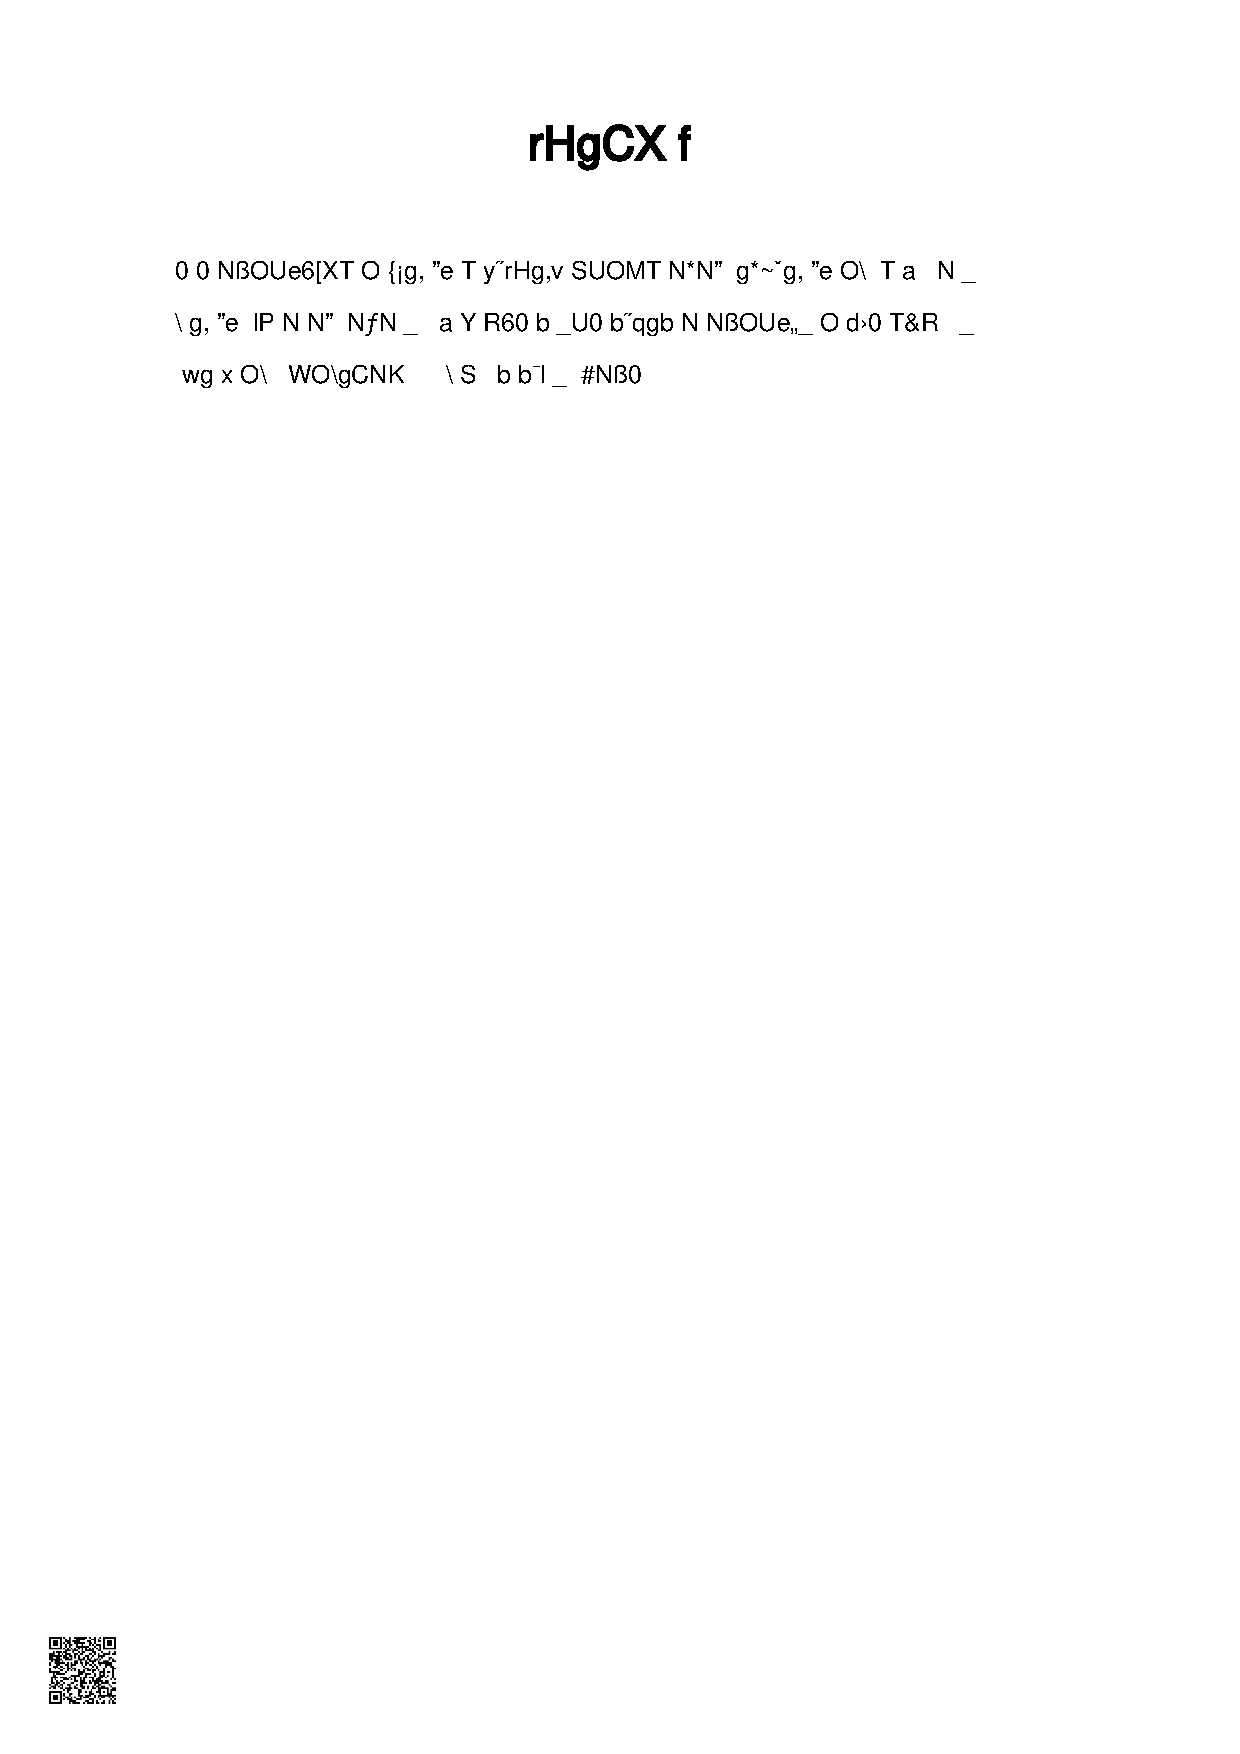
\includegraphics[height = 1.2448\textheight]{img/bqsm_180xxxxxxx.pdf}
    }
\end{textblock}

% vim:ts=4:sw=4

	\cleardoublepage
	\pagestyle{plain}
	\setcounter{page}{0}
	\pagenumbering{Roman}
	\begin{cabstract}
如课业目标所示,学生在第一章为论文精读选择 IEEE Transactions on Pattern Analysis and Machine Intelligence 与 IEEE Journal on Selected Areas in Communications 为来源的当年度期刊进行阅读、第二章为文献管理工具的使用与实测,学生从时下 Endnote、Mendeley、Zotero、Citavi、Papers 等任一种软体选择出符合工作需求流程的工具,在此学生选择Zotero 并写出使用跟操作流程,并且使用指定的来源搜集文献,其来源如 IEEE 、IET 、ACM、Springer、Elsevier、Google 学术、Beidu 学术,并置入于该作业的参考文献中来完成 LaTeX 的北京大学论文格式,第三章则是简述说明 Overleaf 与 LaTeX 的方案与期末学习的总结,最后的章节则是用表格整理本作业所搜集的文献。

\end{cabstract}

%\begin{eabstract}
%    英文摘要部分...
%\end{eabstract}

% vim:ts=4:sw=4

	\tableofcontents
	% 如有需要使用主要符号对照表
	\begin{denotation}

\item[$x,y,m,n,t$] 标量,通常为变量
\item[$K,L,D,M,N,T$] 标量,通常为超参数
\item[$x\in \mathbb{R}^{D}$] D维列向量
\item[$(x_1,\cdots,x_D)$] D维行向量
\item[$(x_1,\cdots,x_D)^T$ or $(x_1;\cdots;x_D)^T$]  D维行向量
\item[$x\in \mathbb{R}^{KD}$]  ($KD$)维的向量
\item[$\mathbb{M}_i$ or $\mathbb{M}_i(\v x)$]  第$i$列为$\v 1$(或者$\v x$),其余为$\v 0$的矩阵
\item[$diag(\v x)$]  对角矩阵,其对角元素为$\v x$
\item[$\v I_N$ or $I$]  ($N\times N$)的单位阵
\item[$\v A \in \mathbb{R}^{D_1\times D_2\times \cdots \times D_K}$]  大小为$D_1\times D_2\times \cdots \times D_K$的张量
\item[$\{x^{(n)}\}^{N}_{n=1}$]  集合
\item[$\{(x^{(n)},y^{(n)})\}^{N}_{n=1}$]  数据集
\item[$\mathcal{N}(\v x;\mu,\sum)$]  变量$x$服从均值为$\mu$,方差为$\sum$的高斯分布

\end{denotation}

\footnotetext[1]{本符号对照表内容选自\citeauthor{qiu2020nndl}老师的《神经网络与深度学习》\cite{qiu2020nndl}一书。}


	\mainmatter
	\chapter{作业目标}
\label{chap:1}

\section{作业说明}

该作业为人工智慧期末报告,其专案为 kancheng/kan-cs-report-in-2021 ,程式码则可于 kan-cs-report-in-2021/AI/pytorch-transformer/code 中查询,而文件则可由专案中进行查询。

\section{论文作业目标}

Step 1 : Read the paperվAttention is all you needտand write a reading report. 

Step 2: Read and run Transformer-related code (NLP Harvard).

Recording the operation result and your understanding in the experimental report.

Step 3: You can choose a specific area (No restriction on direction), and apply the transformer to this area.

It is necessary to find a published paper and successfully reproduce the corresponding result in the paper.Recording the related paper, experimental steps, and your results vs results in the paper to the experimental report.

Step 4: 

The reading report \& source code \& the related paper \& experimental report will be organized and submitted. 


\section{The Annotated Transformer}


Q1: NO GPU available

\begin{itemize}
\item A1: a survey about transformer
\item Example: https://arxiv.org/pdf/1809.02165.pdf
\end{itemize}


Q2: code plagiarism

\begin{itemize}
\item In particular, all code and documentation should be entirely your own work. You may consult with other students about high-level design strategies related to programming assignments, but you may not copy code or use the structure or organization of another student's program.
\item If you use any code or functions found from the internet, please tell us the reference link and how do you use it. Direct code copy from the internet would be considered violation of this policy.
\item If we find there are two returned assignments same in large proportional code, both of the assignments would be considered violation of this policy.
\end{itemize}


	\chapter{论文精读}
\label{chap:2}

此章为 Transformer 模型的 Attention Is All You Need \cite{vaswani2017attention} 与当中阅读论文与心得 :
% \cite{garcia2020admd}

\section{论文精读资讯}

下列论文资讯在 arXiv 为 1706.03762。

\begin{Verbatim}
Attention Is All You Need

Ashish Vaswani, Noam Shazeer, Niki Parmar, Jakob Uszkoreit, Llion Jones, 
Aidan N. Gomez, Lukasz Kaiser, Illia Polosukhin

https://arxiv.org/abs/1706.03762

Comments: 15 pages, 5 figures

Subjects: Computation and Language (cs.CL); Machine Learning (cs.LG)

Cite as: arXiv:1706.03762 [cs.CL] (or arXiv:1706.03762v5 [cs.CL] for this version)
\end{Verbatim}

\section{论文心得}

而论文心得必须根据 IMRAD 的方式进行撰写,其流程分别为四部分,分别为前言(Introduction)、方法(Methods)、结果(Results)和讨论(Discussion),最后则是根据原论文架构的范例,该心得则根据 IMRAD 来分析。

\subsection{前言}

该篇研究根据过往研究成果进行研究,将其发展成新的方法与架构,该方法在各个领域上具有显著的效果,研究者发现循环神经网络(Recurrent neural networks),特别是 Sepp Hochreiter et al. 的长短期记忆(long short-term memory) 和 Junyoung Chung et al. 的门控循环 (gated recurrent) 神经网络,已成为序列建模和转导问题,并且是语言建模和机器翻译中的最先进方法。

此后许多研究者们的努力如 Yonghui Wu et al.、Minh-Thang Luong et al.、Rafal Jozefowicz et al. 继续推动循环语言模型和编码器-解码器架构的界限,而循环模型 (Recurrent models) 通常沿输入和输出序列的符号位置因子计算。将位置与计算时间中的步骤对齐,它们生成一系列隐藏状态 ht,作为先前隐藏状态 ht1 和位置 t 的输入的函数。此固有的顺序性质排除了训练示例中的并行化,这在更长的序列长度时变得至关重要,因为记忆体限制了跨示例的批处理,近来的工作通过分解技巧 Oleksii Kuchaiev et al. 和条件计算 Noam Shazeer et al. 显著提高了计算效率,同时在后者的情况下也提高了模型性能。然而顺序计算的基本约束仍然存在,而且注意机制已成为各种任务中引人注目的序列建模和转导模型的组成部分,允许对依赖项进行建模,而无需考虑它们在输入或输出序列中的距离 Dzmitry Bahdanau et al. 、Yoon Kim et al.,然而除了少数情况如 Ankur Parikh et al.,在所有情况下该注意力机制都与循环网络结合使用。在这项工作中,我们提出了名为 Transformer 的一种避免重复的模型架构,而是完全依靠注意力机制来绘制输入和输出之间的全局依赖关系,而 Transformer 允许显著更多的并行化,并且在八个 P100 GPU 上进行了短短 12 小时的训练后,可以在翻译质量方面达到新的水平。

\subsection{方法}

该研究的模型架构,其大多数具有竞争力的神经序列转导模型都具有编码器-解码器结构,在此研究者编码器将符号表示的输入序列 x 映射到连续表示的序列 z 。同时给定 z 解码器,然后生成一个符号的输出序列 y 后,输出一次一个元素。在每一步过程中,模型都是自回归的 Alex Graves et al.,且在生成下一个时,将先前生成的符号作为额外的输入使用。 Transformer 遵循这一整体架构,使用堆叠的自注意力和逐点、完全连接的编码器和解码器层。

该章节分别分为编码器和解码器堆栈 (Encoder and Decoder Stacks)部分,而注意力 (Attention) 的部分则包含缩放点积注意力 (Scaled Dot-Product Attention) 、多头注意力(Multi-Head Attention) 跟注意力在该研究模型中的应用,同时说明该研究的位置前馈网络 (Position-wise Feed-Forward Networks)、位置前馈网络(Position-wise Feed-Forward Networks)、嵌入和 Softmax (Embeddings and Softmax) 与位置编码 (Positional Encoding)。

\subsection{结果}

在此研究者说明何谓自我注意 (Self-Attention)与训练机制,研究者将自注意力层的各个方面与通常用于将一个可变长度的符号表示序列 x 映射到另一个等长序列 z,例如典型序列转导编码器或解码器中的隐藏层。

过程中考虑了三个需求,首先是每层的总计算复杂度,另一个则是可以并行化的计算量,通过所需的最小顺序操作数来衡量,第三个是网络中远程依赖之间的路径长度,而且当中学习远程依赖是许多序列转导任务中的关键挑战,另外影响学习这种依赖性能力的一个关键因素是前向和后向信号必须在网络中穿越的路径长度,当中输入和输出序列中任意位置组合之间的这些路径越短,而学习远程依赖关系就越容易 Sepp Hochreiter et al.。同时研究者还比较了由不同层类型组成的网络中任意两个输入和输出位置之间的最大路径长度,另外个人注意力不仅清楚地学习执行不同的任务,而且许多人似乎表现出与句子的句法和语义结构相关的行为。

而训练的部分则描述了模型的训练机制并对硬体和优化器 (Optimizer) 与正则化 (Regularization) 进行说明,同时在研究者的训练数据和批处理 (Training Data and Batching),研究者在包含约 450 万个句子对的标准 WMT 2014 英德数据集上进行了训练,同时对句子使用字节对编码进行编码,使它具有大约 37000 个标记的共享源目标词汇表。对于英法转换,研究者使用了明显更大的 WMT 2014 英法数据集,该数据集由 3600 万个句子组成,并将标记拆分为 32000 个单词词表,而句子对按近似序列长度分批在一起,此外每个训练批次包含一组句子对,其中包含大约 25000 个源标记和 25000 个目标标记。

\subsection{讨论}

根据整个研究的工作,该研究者们提出了 Transformer,这是第一个完全基于注意力的序列转换模型,使用多头自注意力取代了编码器-解码器架构中最常用的循环层。而面对翻译任务,当中 Transformer 的训练速度明显快于基于循环或卷积层的架构。另外在 WMT 2014 English-to-German 和 WMT 2014 English-to-French 翻译任务过程中,研究者达到了最先进的水平。

\section{论文翻译}

在此根据论文 Learning with Privileged Information via Adversarial Discriminative Modality Distillation 的章节结构进行翻译,其论文题目的中文字面意义上为通过对抗性判别模态蒸馏(Adversarial Discriminative Modality Distillation) 学习特权资讯 (Privileged Information)。该根据原研究论文架构来分配章节,该篇研究的论文程式码可于 GitHub 专案
取得 (https://github.com/pmorerio/admd)。

\subsection{摘要}
%Abstract 摘要

主导序列转导模型基于复杂的循环或卷积神经网络,包括编码器和解码器,当中性能最好的模型还通过注意力机制连接编码器和解码器。我们提出了一种新的简单网络架构,即 Transformer,它完全基于注意力机制,完全消除了递归和卷积,在两个机器翻译任务上的实验表明,这些模型在质量上更胜一筹,同时更可并行化并且需要更少的训练时间。我们的模型在 WMT 2014 英德翻译任务上达到了 28.4 BLEU,比现有的最佳结果(包括集成)提高了 2 BLEU,而在 WMT 2014 英语到法语翻译任务中,我们的模型在 8 个 GPU 上训练 3.5 天后建立了一个新的单模型最先进的 BLEU 分数 41.8,这是最好的训练成本的一小部分 文献中的模型。最后我们表明,通过将 Transformer 成功应用于具有大量和有限训练数据的英语选区解析,可以很好地推广到其他任务。

\subsection{前言}
% 1 INTRODUCTION 前言

发现循环神经网络(Recurrent neural networks),特别是 Sepp Hochreiter et al. 的长短期记忆(long short-term memory) 和 Junyoung Chung et al. 的门控循环 (gated recurrent) 神经网络,已成为序列建模和转导问题,并且是语言建模和机器翻译中的最先进方法。

此后许多研究者们的努力如 Yonghui Wu et al.、Minh-Thang Luong et al.、Rafal Jozefowicz et al. 继续推动循环语言模型和编码器-解码器架构的界限,而循环模型 (Recurrent models) 通常沿输入和输出序列的符号位置因子计算。将位置与计算时间中的步骤对齐,它们生成一系列隐藏状态 ht,作为先前隐藏状态 ht1 和位置 t 的输入的函数。此固有的顺序性质排除了训练示例中的并行化,这在更长的序列长度时变得至关重要,因为记忆体限制了跨示例的批处理,近来的工作通过分解技巧 Oleksii Kuchaiev et al. 和条件计算 Noam Shazeer et al. 显著提高了计算效率,同时在后者的情况下也提高了模型性能。然而顺序计算的基本约束仍然存在,而且注意机制已成为各种任务中引人注目的序列建模和转导模型的组成部分,允许对依赖项进行建模,而无需考虑它们在输入或输出序列中的距离 Dzmitry Bahdanau et al. 、Yoon Kim et al.,然而除了少数情况如 Ankur Parikh et al.,在所有情况下该注意力机制都与循环网络结合使用。在这项工作中,我们提出了名为 Transformer 的一种避免重复的模型架构,而是完全依靠注意力机制来绘制输入和输出之间的全局依赖关系,而 Transformer 允许显著更多的并行化,并且在八个 P100 GPU 上进行了短短 12 小时的训练后,可以在翻译质量方面达到新的水平。

\subsection{背景}
% 2 背景

减少顺序计算的目标也构成了 Lukasz Kaiser et al. 的扩展神经 GPU、Nal Kalchbrenner et al. 的 ByteNet 和 Jonas Gehring et al. 的 ConvS2S 基础,所有这些都使用卷积神经网络作为基本构建块,并行计算所有输入和输出位置。在这些模型中,其关联来自两个任意输入或输出位置的信号所需的操作数量随着位置之间的距离而增加,对于 ConvS2S 是线性增长,对于 ByteNet 是对数增长。这使得学习远距离位置之间的依赖关系变得更加困难 Sepp Hochreiter et al.,在 Transformer 中,这被减少到恒定数量的操作,尽管代价是由于平均注意力加权位置而导致有效分辨率降低,我们用多头注意力来抵消这种影响,如第 3.2 节所述。自注意 (Self-attention) 有时也称为内注意 (intra-attention),这是一种将单个序列的不同位置关联起来以计算序列表示的注意机制,而自注意力已成功用于各种任务,包括阅读理解、抽象摘要、文本蕴涵和学习与任务无关的句子表示上 Jianpeng Cheng et al.、 Ankur Parikh et al.、 Romain Paulus et al.、 Zhouhan Lin et al.。而端到端记忆网络基于循环注意机制而不是序列对齐循环,并且已被证明在简单语言问答和语言建模任务上表现良好 Sainbayar Sukhbaatar et al.,然而据我们所知 Transformer 是第一个完全依赖自注意力来计算其输入和输出表示而不使用序列对齐 RNN 或卷积的转换模型。在接下来的部分中,我们将描述 Transformer,激发自我注意并讨论它相对于 Lukasz Kaiser et al.、 Nal Kalchbrenner et al. 和 Jonas Gehring et al. 等模型的优势。

\subsection{模型架构}
% 3 

大多数具有竞争力的神经序列转导模型都具有编码器-解码器结构 Kyunghyun Cho et al.、 Dzmitry Bahdanau et al.、Ilya Sutskever et al.。在此编码器将符号表示的输入序列 $(x_{1}, ..., x{n})$ 映射到连续表示的序列 $\mathbf{z}=\left(z_{1}, \ldots, z_{n}\right)$。给定 $\mathbf{z}$ 解码器然后生成一个符号的输出序列 $(y_{1}, ..., y{m})$,一次一个元素。在每一步其模型都是自回归的 Alex Graves et al.,在生成下一个时会将先前生成的符号作为额外的输入使用。 Transformer 遵循这一整体架构,使用堆叠的自注意力和逐点、完全连接的编码器和解码器层,分别如图 1 的左半部分和右半部分所示。

\begin{figure}[htb]
\centering 
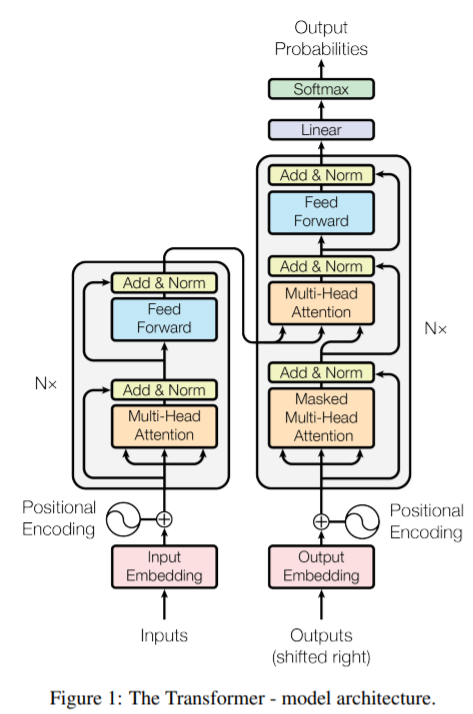
\includegraphics[width=0.6\textwidth]{img/tm1.png} 
\caption{The Transformer - 模型架構 (model architecture)}
\label{Test}
\end{figure}

1. 編碼器和解碼器堆棧 (Encoder and Decoder Stacks)

編碼器 (Encoder): 編碼器由 N = 6 個相同層的堆棧組成,每層有兩個子層,第一個是多頭自注意力機制,第二個是簡單的、位置明智的全連接前饋網絡,我們在兩個子層的每一個周圍都使用了一個殘差連接 Kaiming He et al. ,然後是層歸一化 Jimmy Lei Ba et al.。即每個子層的輸出是 $LayerNorm(x + Sublayer(x))$,其中 $Sublayer(x)$ 是子層自己實現的函數,為了促進這些殘差連接,模型中的所有子層以及嵌入層產生維度 $d_{model}$ = 512 的輸出。

解碼器 (Decoder): 解碼器也由 N = 6 個相同層的堆棧組成。除了每個編碼器層中的兩個子層之外,解碼器還插入了第三個子層,該子層對編碼器堆棧的輸出執行多頭注意。而與編碼器類似,我們在每個子層周圍使用殘差連接,然後進行層歸一化,我們還修改了解碼器堆棧中的自註意子層,以防止位置關注後續位置,這種掩碼與輸出嵌入偏移一個位置的事實相結合,確保位置 i 的預測只能依賴於小於 i 位置的已知輸出。

2. 注意力 (Attention)

注意力函数可以描述为将查询和一组键值对映射到输出,其中查询、键、值和输出都是向量。输出计算为值的加权总和,其中分配给每个值的权重由查询与相应键的兼容性函数计算。

\begin{figure}[htb]
\centering 
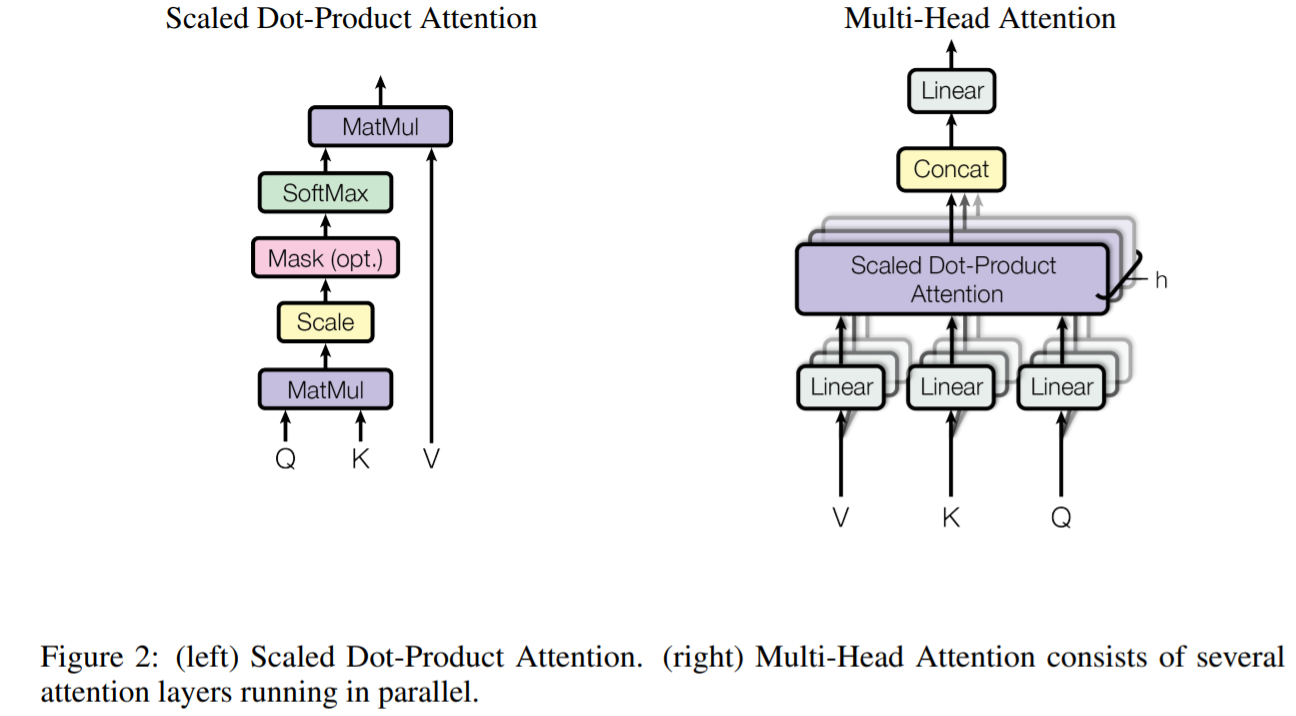
\includegraphics[width=0.95\textwidth]{img/tm2.png} 
\caption{缩放的点积注意力和多头注意力}
\label{Test}
\end{figure}

图 2:(左)缩放的点积注意力。 (右)多头注意力由多个并行运行的注意力层组成。缩放点积注意力 (Scaled Dot-Product Attention)、多头注意力 (Multi-Head Attention)。

(1) 缩放点积注意力 (Scaled Dot-Product Attention)

我们将我们的特别关注称为“Scaled Dot-Product Attention”(图 2),输入包括维度 $d_{k}$ 的查询和键,以及维度 $d_{v}$ 的值,我们使用所有键计算查询的点积,将每个键除以 $sqrt{d_{k}}$ ,并应用 softmax 函数来获得值的权重。在实践中我们同时计算一组查询的注意力函数,将它们打包成一个矩阵 $Q$,键和值也一起打包成矩阵 $K$ 和 $V$,其键和值也一起打包成矩阵 $K$ 和 $V$ 。其计算的矩阵输出为 :

\begin{equation}
\operatorname{Attention}(Q, K, V)=\operatorname{softmax}\left(\frac{Q K^{T}}{\sqrt{d_{k}}}\right) V
\end{equation}

两个最常用的注意力函数是加的注意力 Dzmitry Bahdanau et al. 和点积乘的注意力,除了 $\frac{1}{\sqrt{d{k}}}$ 的缩放因子之外,点积注意力与我们的方法相同。加法的注意力使用上具有单个隐藏层的前馈网络计算兼容性函数,虽然两者在理论复杂度上相似,但点积注意力在实践中速度更快,空间效率更高,因为它可以使用高度优化的矩阵乘法程式码来实现。虽然对于较小的 $d_{k}$ 值,这两种机制的表现相似,但加法注意力优于点积注意力,而无需针对较大的 $d_{k}$ 值进行缩放 Denny Britz et al.,我们怀疑对于较大的 $d_{k}$ 值,点积的量级会变大,从而将 softmax 函数推入梯度极小的区域 \footnote{为了说明点积变大的原因,假设 $q$ 和 $k$ 的分量是均值为 0 且方差为 1 的独立随机变量,那么他们的点积 $q \cdot k=\sum_{i=1}^{a_{k}} q_{i} k_{i}$,均值为 0,方差为 $d_{k}$。},为了抵消这种影响,我们通过 $\frac{1}{\sqrt{d{k}}}$ 缩放点积。

(2) 多头注意力 (Multi-Head Attention)

我们发现,与使用 $d_{model}$ 维度的键、值和查询执行单个注意力函数不同,我们发现将查询、键和值分别线性投影到 $d_{k}$、$d_{k}$ 和 $d_{v}$ 维度的不同学习线性投影 $h$ 次是有益的。然后在查询、键和值的这些投影版本中的每一个上,我们并行执行注意力功能,产生 $d_{v}$ 维输出值。这些被连接并再次投影,从而产生最终值,如图 2 所示。

$$\operatorname{MultiHead}(Q, K, V) \&=\operatorname{Concat}\left(\text { head }_{1}, \ldots, \text { head }_{\mathrm{h}}\right) W^{O} $$
\begin{equation}
\text {head}_{\mathrm{i}} \&=\operatorname{Attention}\left(Q W_{i}^{Q}, K W_{i}^{K}, V W_{i}^{V}\right)
\end{equation}

其中投影是参数矩阵 $W_{i}^{Q} \in \mathbb{R}^{d_{\text {model }} \times d_{k}}, W_{i}^{K} \in \mathbb{R}^{d_{\text {model }} \times d_{k}}, W_{i}^{V} \in \mathbb{R}^{d_{\text {model }} \times d_{v}}$ and $W^{O} \in \mathbb{R}^{h d_{v} \times d_{\text {model }}}$。在这项工作中,我们使用了 $h = 8$ 个平行的注意力层或头部。对于每一个,我们使用 $d_{k} = d_{v} = d_{model}/h = 64$,由于每个头部的维数减少,总的计算成本与全维的单头注意力相似。


(3) 注意力在我们模型中的应用 (Applications of Attention in our Model)

Transformer 以三种不同的方式使用多头注意力:

\begin{itemize}
\item [-] 在"编码器-解码器注意力" 层中,查询来自前一个解码器层,记忆键和值来自编码器的输出,这允许解码器中的每个位置都参与输入序列中的所有位置,这模仿了序列到序列模型中典型的编码器-解码器注意力机制,例如 Yonghui Wu et al.、 Dzmitry Bahdanau et al.、 Jonas Gehring et al.。

\item [-] 编码器包含自注意层,在自注意力层中,所有的键、值和查询都来自同一个地方,在这种情况下是编码器上一层的输出。编码器中的每个位置都可以参与编码器前一层中的所有位置。

\item [-] 类似地,解码器中的自注意力层允许解码器中的每个位置关注解码器中直到并包括该位置的所有位置,而我们需要防止解码器中的左向信息流以保留自回归特性。我们通过屏蔽 (设置为 $-\infty$) softmax 输入中与非法连接相对应的所有值来在缩放点积注意力内部实现这一点。 See Figure 2.
\end{itemize}

3. 位置前馈网络 (Position-wise Feed-Forward Networks)

除了注意力子层之外,我们的编码器和解码器中的每一层都包含一个完全连接的前馈网络,该网络分别且相同地应用于每个位置,这由两个线性变换组成,中间有一个 ReLU 激活。

\begin{equation}
\mathrm{FFN}(x)=\max \left(0, x W_{1}+b_{1}\right) W_{2}+b_{2}
\end{equation}

虽然不同位置的线性变换是相同的,但它们在层与层之间使用不同的参数。另一种描述方式是两个卷积核大小为 1。输入输出维数 $d_{model} = 512$,内层维数 $d_{ff} = 2048$。

4. 嵌入和 Softmax (Embeddings and Softmax)

其他序列转导模型类似,我们使用学习嵌入将输入标记和输出标记转换为维度 $d_{model}$ 的向量,我们还使用通常学习的线性变换和 softmax 函数将解码器输出转换为预测的下一个标记概率。在我们的模型中,我们在两个嵌入层和 pre-softmax 线性变换之间共享相同的权重矩阵,类似于 Ofir Press et al.,在嵌入层中,我们将这些权重乘以 $\sqrt{d_{model}}$。

5. 位置编码 (Positional Encoding)

由于我们的模型不包含递归和卷积,为了让模型利用序列的顺序,我们必须注入一些关于标记在序列中的相对或绝对位置的信息,为此我们将“位置编码”添加到编码器和解码器堆栈底部的输入嵌入中。位置编码与嵌入具有相同的维度 $d_{model}$ 因此可以将两者相加,位置编码有多种选择,学习和固定 Jonas Gehring et al.。

表 1:不同层类型的最大路径长度、每层复杂度和最小顺序操作数, $n$ 是序列长度、 $d$ 是表示维度、 $k$ 是卷积核大小, $r$ 是受限自注意力中的邻域大小。

\begin{figure}[htb]
\centering 
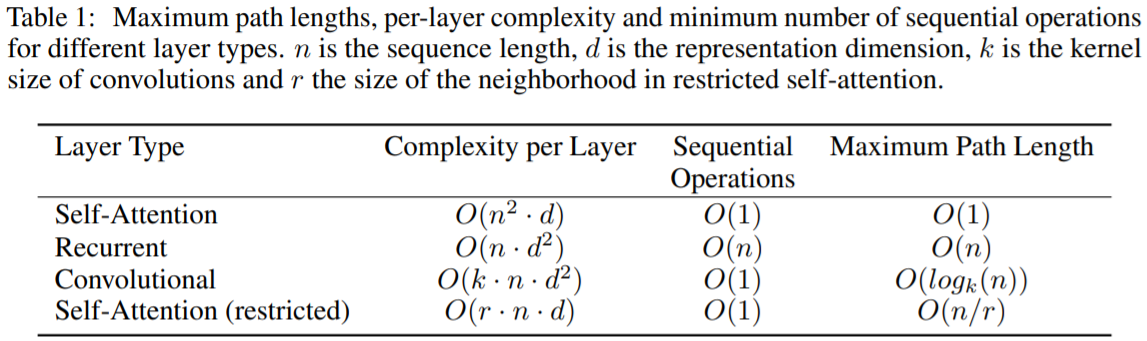
\includegraphics[width=0.95\textwidth]{img/t1.png} 
\caption{不同层类型的最大路径长度、每层复杂度和最小顺序操作数}
\label{Test}
\end{figure}

在這項工作中,我們使用不同頻率的正弦和余弦函數:

\begin{equation}
\begin{aligned}
P E_{(p o s, 2 i)} &=\sin \left(\operatorname{pos} / 10000^{2 i / d_{\text {model }}}\right) \\
P E_{(p o s, 2 i+1)} &=\cos \left(\operatorname{pos} / 10000^{2 i / d_{\text {model }}}\right)
\end{aligned}
\end{equation}

其中 pos 是位置,i 是维度。也就是说,位置编码的每个维度对应一个正弦曲线。波长形成从 $2\pi$ 到 $10000 \cdot 2 \pi$ 的几何级数。我们选择这个函数是因为我们假设它可以让模型很容易地学习通过相对位置来参与,因为对于任何固定的偏移量 $k$,$PE_{pos+k}$ 可以表示为 $PE_{pos}$ 的线性函数。我们还尝试使用学习的位置嵌入 Jonas Gehring et al.,发现两个版本产生了几乎相同的结果 (见表 3 行 (E)),我们选择了正弦版本,因为它可能允许模型外推到比训练期间遇到的序列长度更长的序列长度。

\subsection{Why Self-Attention}

在本节中,我们将自注意力层的各个方面与通常用于将一个可变长度的符号表示序列 $(x_{1}, ..., x_{n})$ 映射到另一个等长序列 $(z_{1}, ..., z_{n})$, 与 $x_{i}, z_{i} \in \mathbb{R}^{d}$,例如典型序列转导编码器或解码器中的隐藏层。为了激发我们使用自注意力,我们考虑了三个需求。一个是每层的总计算复杂度。另一个是可以并行化的计算量,通过所需的最小顺序操作数来衡量。第三个是网络中远程依赖之间的路径长度。学习远程依赖是许多序列转导任务中的关键挑战,影响学习这种依赖性能力的一个关键因素是前向和后向信号必须在网络中穿越的路径长度。输入和输出序列中任意位置组合之间的这些路径越短,学习远程依赖关系就越容易 Sepp Hochreiter et al. ,因此我们还比较了由不同层类型组成的网络中任意两个输入和输出位置之间的最大路径长度。如表 1 中所述,自注意力层将所有位置与恒定数量的顺序执行操作连接起来,而循环层需要 $O(n)$ 顺序操作。在计算复杂度方面,当序列长度 $n$ 小于表示维数 $d$ 时,自注意力层比循环层更快,这是机器翻译中最先进模型使用的句子表示的最常见情况 ,例如词片 Yonghui Wu et al. 和字节对 Rico Sennrich et al. 表示。为了提高涉及非常长序列的任务的计算性能,可以将自注意力限制为仅考虑输入序列中以相应输出位置为中心的大小为 $r$ 的邻域。这会将最大路径长度增加到 $O(n=r)$ ,我们计划在未来的工作中进一步研究这种方法。内核宽度 $k < n$ 的单个卷积层不会连接所有输入和输出位置对。这样做需要在连续内核的情况下堆叠 $O(n=k)$ 卷积层,或者在扩张卷积的情况下需要 $O(logk(n))$ Nal Kalchbrenner et al.,增加任意两个位置之间最长路径的长度 在网络中,卷积层通常比循环层成本高 $k$ 倍。然而 Francois Chollet 的可分离卷积将复杂度大大降低到 $O\left(k \cdot n \cdot d+n \cdot d^{2}\right)$。然而即使 $k = n$ 可分离卷积的复杂度也等于自注意力层和逐点前馈层的组合,我们在我们的模型中采用的方法。作为附带好处,self-attention 可以产生更多可解释的模型。我们从我们的模型中检查注意力分布,并在附录中展示和讨论示例。个人注意力不仅清楚地学习执行不同的任务,而且许多人似乎表现出与句子的句法和语义结构相关的行为。

\subsection{训练}

本节描述了我们模型的训练机制。

1. 训练数据和批处理 (Training Data and Batching)

我们在包含约 450 万个句子对的标准 WMT 2014 英德数据集上进行了训练。句子使用字节对编码 Denny Britz et al. 进行编码,它具有大约 37000 个标记的共享源目标词汇表。对于英法,我们使用了明显更大的 WMT 2014 英法数据集,该数据集由 3600 万个句子组成,并将标记拆分为 32000 个单词词表 Yonghui Wu et al.,句子对按近似序列长度分批在一起。每个训练批次包含一组句子对,其中包含大约 25000 个源标记和 25000 个目标标记。

2. 硬体和时间表 (Hardware and Schedule)

我们在一台配备 8 个 NVIDIA P100 GPU 的机器上训练我们的模型,对于我们使用整篇论文中描述的超参数的基本模型,每个训练步骤大约需要 0.4 秒。我们对基本模型进行了总共 100,000 步或 12 小时的训练,对于我们的大型模型 (在表 3 的底线中进行了描述),步进时间为 1.0 秒,大模型训练了 300,000 步 (3.5 天)。


3. Optimizer

我们使用了 Adam 优化器 Diederik Kingma et al.,其中 $\beta_{1}=0.9, \beta_{2}=0.98$ and $\epsilon=10^{-9}$。我们根据以下公式在训练过程中改变学习率:

\begin{equation}
\text { lrate }=d_{\text {model }}^{-0.5} \cdot \min \left(\text { step\_num }^{-0.5}, \text { step\_num } \cdot \text { warmup\_steps }^{-1.5}\right)
\end{equation}

这对应于在第一个 $warmup_steps$ 训练步骤中线性增加学习率,然后与步数的平方根成反比地减少学习率。我们使用了 $warmup\_steps = 4000$。

4. 正则化 (Regularization)

我们在训练期间采用三种类型的正则化:

(1) Residual Dropout 

我们将 Nitish Srivastava 的 dropout 应用于每个子层的输出,然后再将其添加到子层输入中并进行归一化。此外我们将 dropout 应用于编码器和解码器堆栈中的嵌入和位置编码的总和。对于基本模型,我们使用 $P_{drop} = 0.1$ 的比率。

表 2:Transformer 在 English-German 和 English-to-French newstest2014 测试中取得了比之前最先进的模型更好的 BLEU 分数,而训练成本只是其中的一小部分。

\begin{figure}[htb]
\centering 
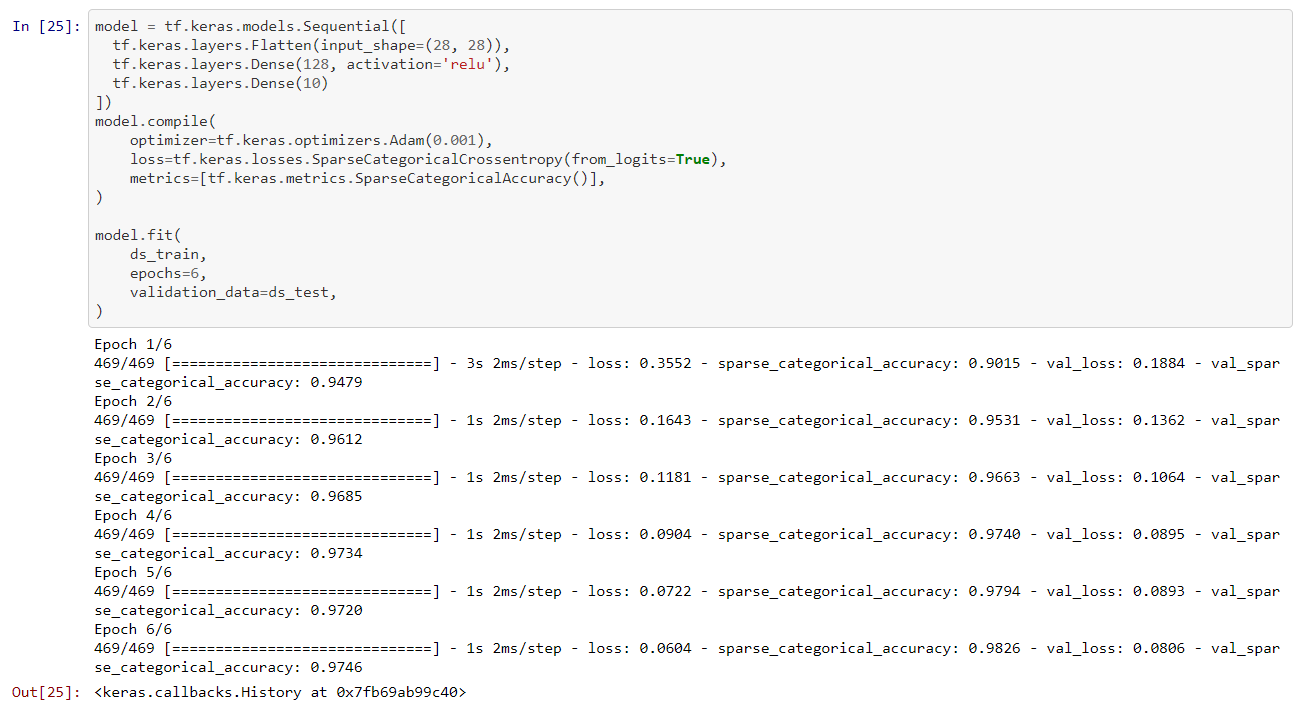
\includegraphics[width=0.95\textwidth]{img/t2.png} 
\caption{:Transformer 在 English-German 和 English-to-French newstest2014}
\label{Test}
\end{figure}

(2) 标签平滑 (Label Smoothing)

在训练期间,我们采用了值 $\epsilon_{l s}=0.1$ Christian Szegedy et al. 的标签平滑,这会降低困惑度,因为模型会变得更加不确定,但会提高准确性和 BLEU 分数。

\subsection{结果}

1. 机器翻译 (Machine Translation)

在 WMT 2014 英德翻译任务中,大转换器模型 (表 2 中的 Transformer (big)) 以超过 2.0 的 BLEU 超过先前报告的最佳模型 (包括集成),建立了一个至今为止最好的 BLEU 分数为 28.4。该模型的配置列在表 3 的底部。在 8 个 P100 GPU 上训练需要 3.5 天,甚至我们的基础模型也超过了所有先前发布的模型和集成模型,其训练成本仅为任何竞争模型的一小部分。在 WMT 2014 英法翻译任务中,我们的大模型达到 41.0 的 BLEU 分数,优于之前发布的所有单个模型,低于之前状态的训练成本 $1/4$ 。为英语到法语训练的 Transformer (大) 模型使用辍学率 $P_{drop} = 0.1$,而不是 0.3。对于基本模型,我们使用了通过平均最后 5 个检查点获得的单个模型,这些检查点以 10 分钟的间隔写入。对于大型模型,我们对最后 20 个检查点进行了平均。我们使用了波束大小为 4 且长度惩罚 $\alpha=0.6$ Yonghui Wu et al. 的波束搜索,这些超参数是在开发集上进行实验后选择的,我们在推理过程中将最大输出长度设置为输入长度 $+ 50$,但在可能的情况下提前终止 Yonghui Wu et al.。表 2 总结了我们的结果,并将我们的翻译质量和训练成本与文献中的其他模型架构进行了比较。我们通过将训练时间、使用的 GPU 数量和每个 GPU 5 的持续单精度浮点容量的估计相乘来估计用于训练模型的浮点运算次数。

2. 型号变化 (Model Variations)

为了评估 Transformer 不同组件的重要性,我们以不同的方式改变了我们的基本模型,测量了开发集 newstest2013 上英德翻译的性能变化,我们使用了前一节中描述的波束搜索,但没有检查点平均。我们在表 3 中展示了这些结果,在表 3 的行 (A) 中,我们改变了注意力头的数量以及注意力键和值维度,保持计算量不变,如第 3.2.2 节所述,虽然单头注意力比最佳设置差 0.9 BLEU,但质量也会随着头数过多而下降。

\begin{figure}[htb]
\centering 
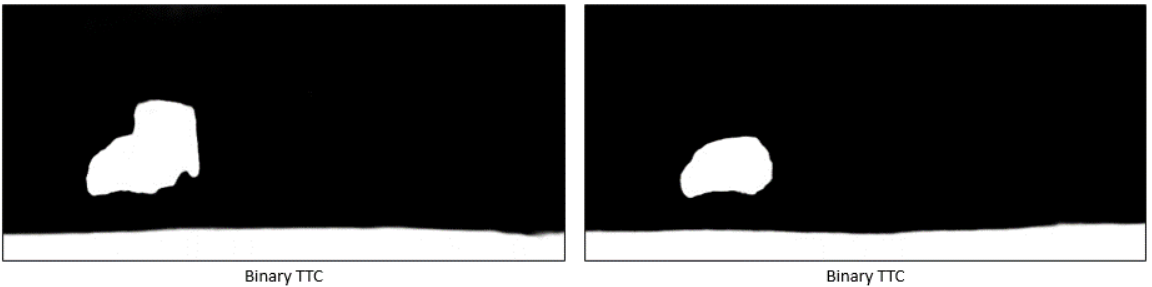
\includegraphics[width=0.95\textwidth]{img/t3.png} 
\caption{Transformer 架构的变化}
\label{Test}
\end{figure}

表 3:Transformer 架构的变化,未列出的值与基本模型的值相同。所有指标都在英语到德语的翻译开发集 newstest2013 上,根据我们的字节对编码,列出的困惑是每个单词的,不应与每个单词的困惑进行比较。

\begin{figure}[htb]
\centering 
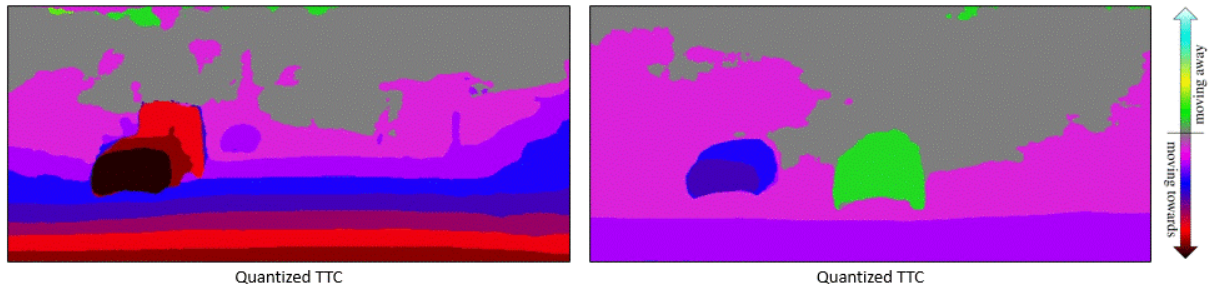
\includegraphics[width=0.95\textwidth]{img/t4.png} 
\caption{Transformer 很好地推广到英语选区解析}
\label{Test}
\end{figure}

表 4:Transformer 很好地推广到英语选区解析 (结果在 WSJ 的第 23 节)在表 3 的行 (B) 中,我们观察到减少注意力密钥大小 $d_{k}$ 会损害模型质量。这表明确定兼容性并不容易,并且比点积更复杂的兼容性函数可能是有益的,我们在行 (C) 和 (D) 中进一步观察到,正如预期的那样,更大的模型更好,并且 dropout 非常有助于避免过度拟合。在行 (E) 中,我们用学习的位置嵌入 Jonas Gehring et al. 替换了我们的正弦位置编码,并观察到与基本模型几乎相同的结果。

3. 英语选区解析 (English Constituency Parsing)

为了评估 Transformer 是否可以推广到其他任务,我们对英语选区解析进行了实验,这项任务提出了具体的挑战:输出受到强大的结构约束,并且明显长于输入。此外 RNN 序列到序列模型无法在小数据机制中获得最先进的结果 Vinyals et al.,我们在 Mitchell P Marcus 的 Penn Treebank 的华尔街日报 (WSJ) 部分训练了一个 $d_{model} = 1024$ 的 4 层转换器,大约有 40K 个训练句子。我们还在半监督环境中对其进行了训练,使用更大的高置信度和 BerkleyParser 语料库,其中包含大约 1700 万个句子 Vinyals et al.,我们在 WSJ only setting 中使用了 16K 标记的词汇表,在半监督设置中使用了 32K 标记的词汇表。我们只进行了少量实验来选择第 22 节开发集上的 dropout、注意力和残差 (第 5.4 节)、学习率和波束大小,所有其他参数与英语到德语基础翻译模型保持不变。在推理过程中,我们将最大输出长度增加到输入长度 $+ 300$,我们仅对 WSJ 和半监督设置使用了 21 和 $\alpha=0.3$的波束大小。我们在表 4 中的结果表明,尽管缺乏针对特定任务的调整,但我们的模型表现出奇的好,产生了比除循环神经网络语法 Chris Dyer et al. 以外的所有先前报告的模型更好的结果。与 RNN 序列到序列模型 Vinyals et al. 相比,即使仅在 WSJ 训练集的 40K 句子上进行训练,Transformer 的性能也优于 Berkeley-Parser Slav Petrov et al.。

\subsection{结论}

在这项工作中,我们提出了 Transformer,这是第一个完全基于注意力的序列转换模型,用多头自注意力取代了编码器-解码器架构中最常用的循环层。对于翻译任务,Transformer 的训练速度明显快于基于循环或卷积层的架构。在 WMT 2014 English-to-German 和 WMT 2014 English-to-French 翻译任务中,我们达到了最先进的水平。在前一个任务中,我们最好的模型甚至优于所有先前报告的集成。我们对基于注意力模型的未来感到兴奋,并计划将它们应用于其他任务。我们计划将 Transformer 扩展到涉及文本以外的输入和输出模式的问题,并研究局部、受限的注意力机制以有效处理大型输入和输出,如图像、音频和影像。减少世代的连续性是我们的另一个研究目标,我们用于训练和评估模型的代码可在 https://github.com/tensorflow/tensor2tensor 上找到。



	\chapter{LaTeX 方案与总结}
\label{chap:3}

\subsection{LaTeX 方案}

由于该作业最后需要使用 LaTeX 进行呈现,在此本作业选择使用 Overleaf 进行开发工具的选项,同时本作业也考虑到之后在不同作业与不同状况下有可能遇到的问题,所以特别进行不同的方案,为之后有可能遇到的状况进行准备。

LaTeX 为一种基于 TeX 而开发的文件排版系统,其优势在于进行编排档时可以进行版控,同时该方案所产生的 PDF 档内容极小,但劣势则是在于在一些情况下,撰写的时间会比较费力,若要符合一般的档需求,则使用目前的文书编辑软件与工具,甚至是商用的在线文书编辑平台来进行工作。当然也有开源跨平台授权的文书软件方案。

在此考虑下,本地端可以考虑使用 Texmaker ,其优势原因在于开源,该软件是专门支持 LaTeX 的图形接口功能,只要事先装好 MiKTeX 等 LaTeX 的开发环境,就可以快速投入工作流程。而 Overleaf 则是商业的多人跨平台协作方案,其最佳的优势在于支持多人协作与版本控制,而且初学者不用考虑到 LaTeX 在本地端较复杂的环境维护,另外 Overleaf 还有许多志愿者所贡献的模板,而本作业就是使用 Overleaf 平台上名为  iofu728 所提供的北京大学硕士论文格式模板。最后回到两者的方案上,前者 Texmaker 可以提供直觉化的图形接口操作,不受网络环境影响的本地端 LaTeX 开发环境,同时后者的 Overleaf 则是在快速开发、多人协作与容易入门上,占有极大的竞争优势,两者相辅相成。

最后整理出使用者在面对 LaTeX 学习门坎最高的数学式跟符号问题,在此有三种可以辅助的方式,其一为 Mathpix Snip 的 OCR 辨识转 LaTeX 的数学式符号输出,该方案需要注册平台后,其使用者就可以使用指定的版本,此外在 Texmaker 当中就有特定符号的图形化接口操作,而目前 MS Office 2019 版本在数学式上也有支持 LaTeX 的转换,虽然在一些细节上处理并没有很好,但是已经可以面对大量的工作量需求。


\begin{figure}[htb]
\centering 
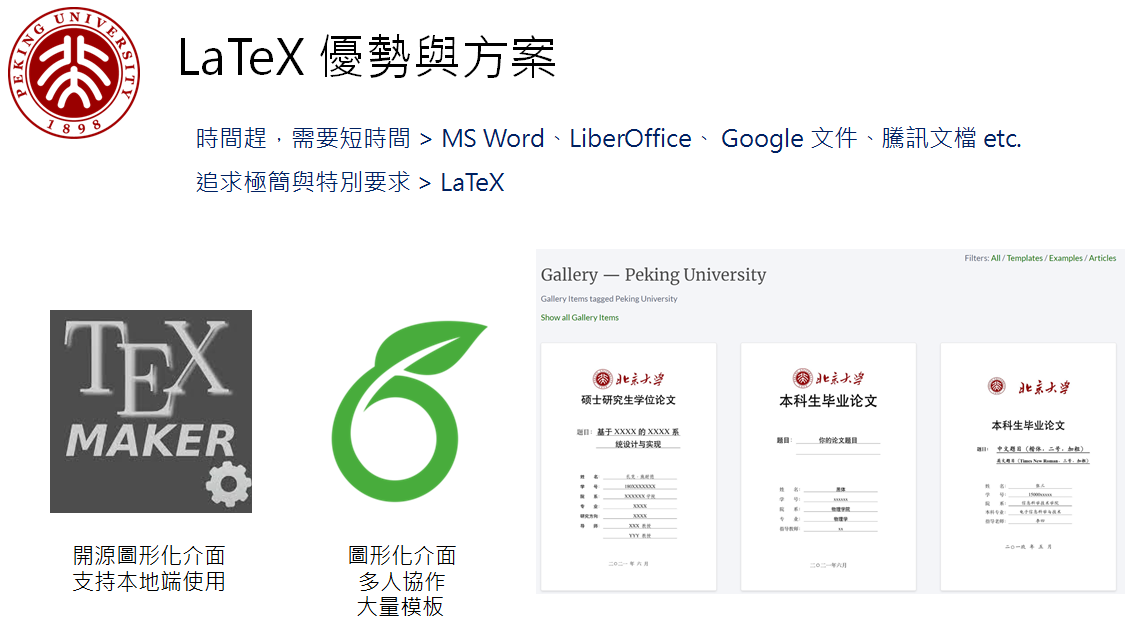
\includegraphics[width=0.90\textwidth]{img/c3m0.png} 
\caption{LaTeX 的方案}
\label{Test}
\end{figure}

\begin{figure}[htb]
\centering 
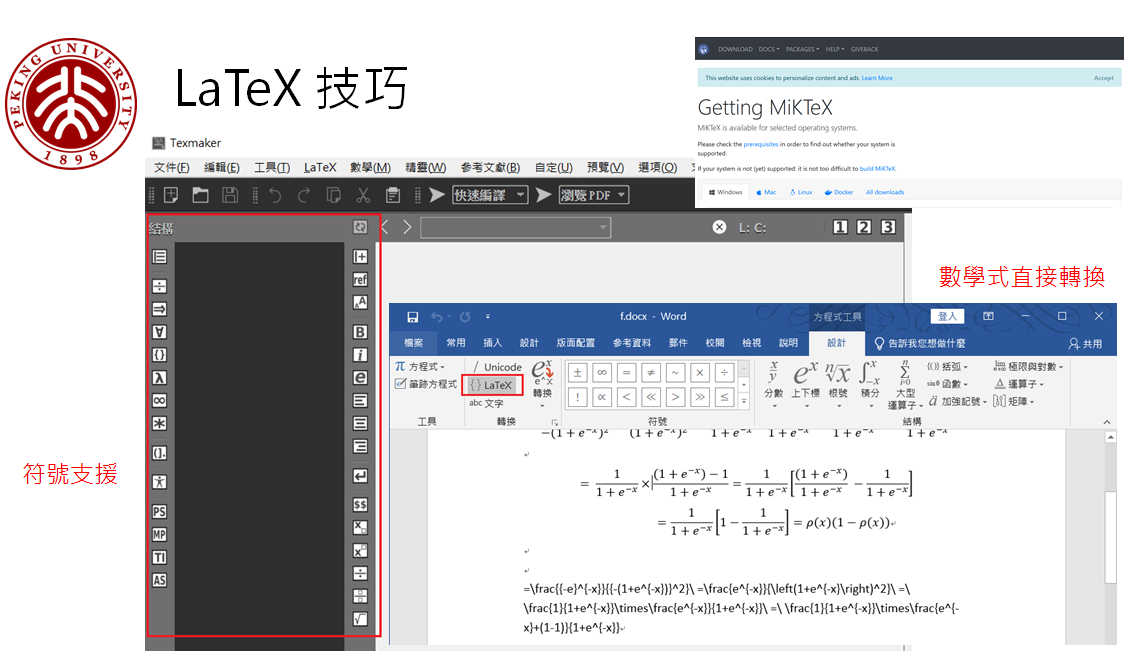
\includegraphics[width=0.90\textwidth]{img/c3m1.png} 
\caption{LaTeX 的快速加工}
\label{Test}
\end{figure}

\begin{figure}[htb]
\centering 
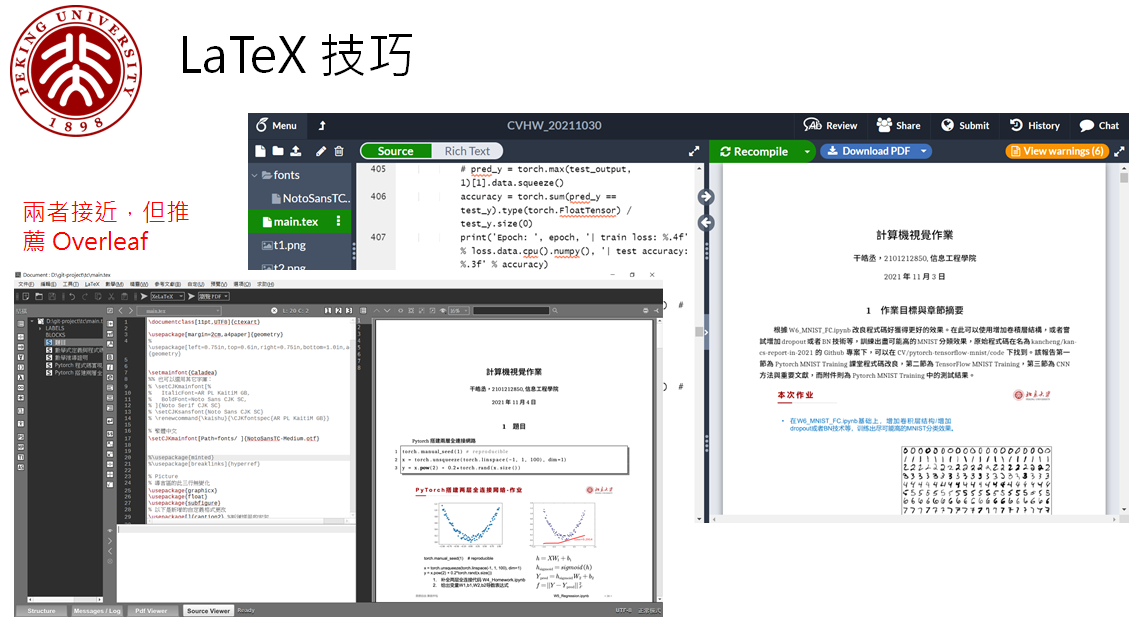
\includegraphics[width=0.90\textwidth]{img/c3m2.png} 
\caption{LaTeX 方案比較}
\label{Test}
\end{figure}

\begin{figure}[htb]
\centering 
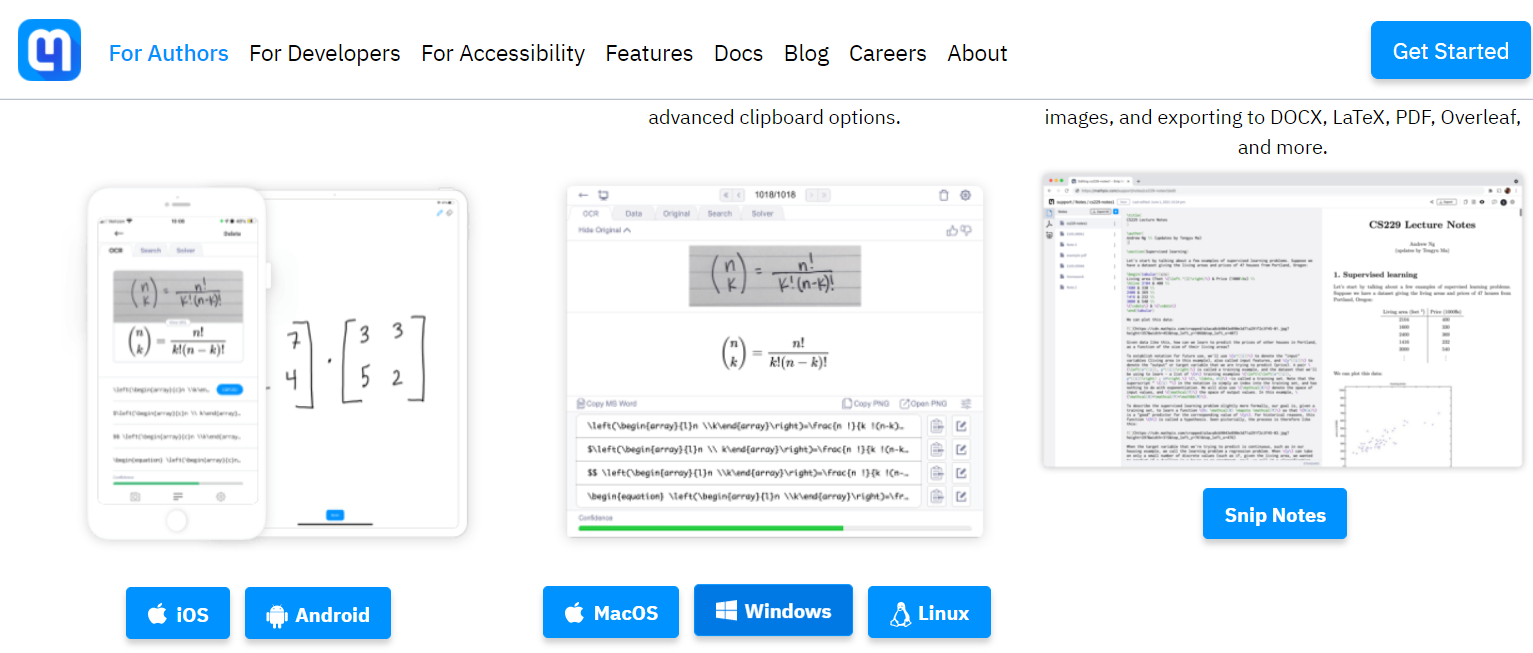
\includegraphics[width=0.90\textwidth]{img/c3m3.png} 
\caption{Mathpix Snip 的 LaTeX 方案}
\label{Test}
\end{figure}

\begin{figure}[htb]
\centering 
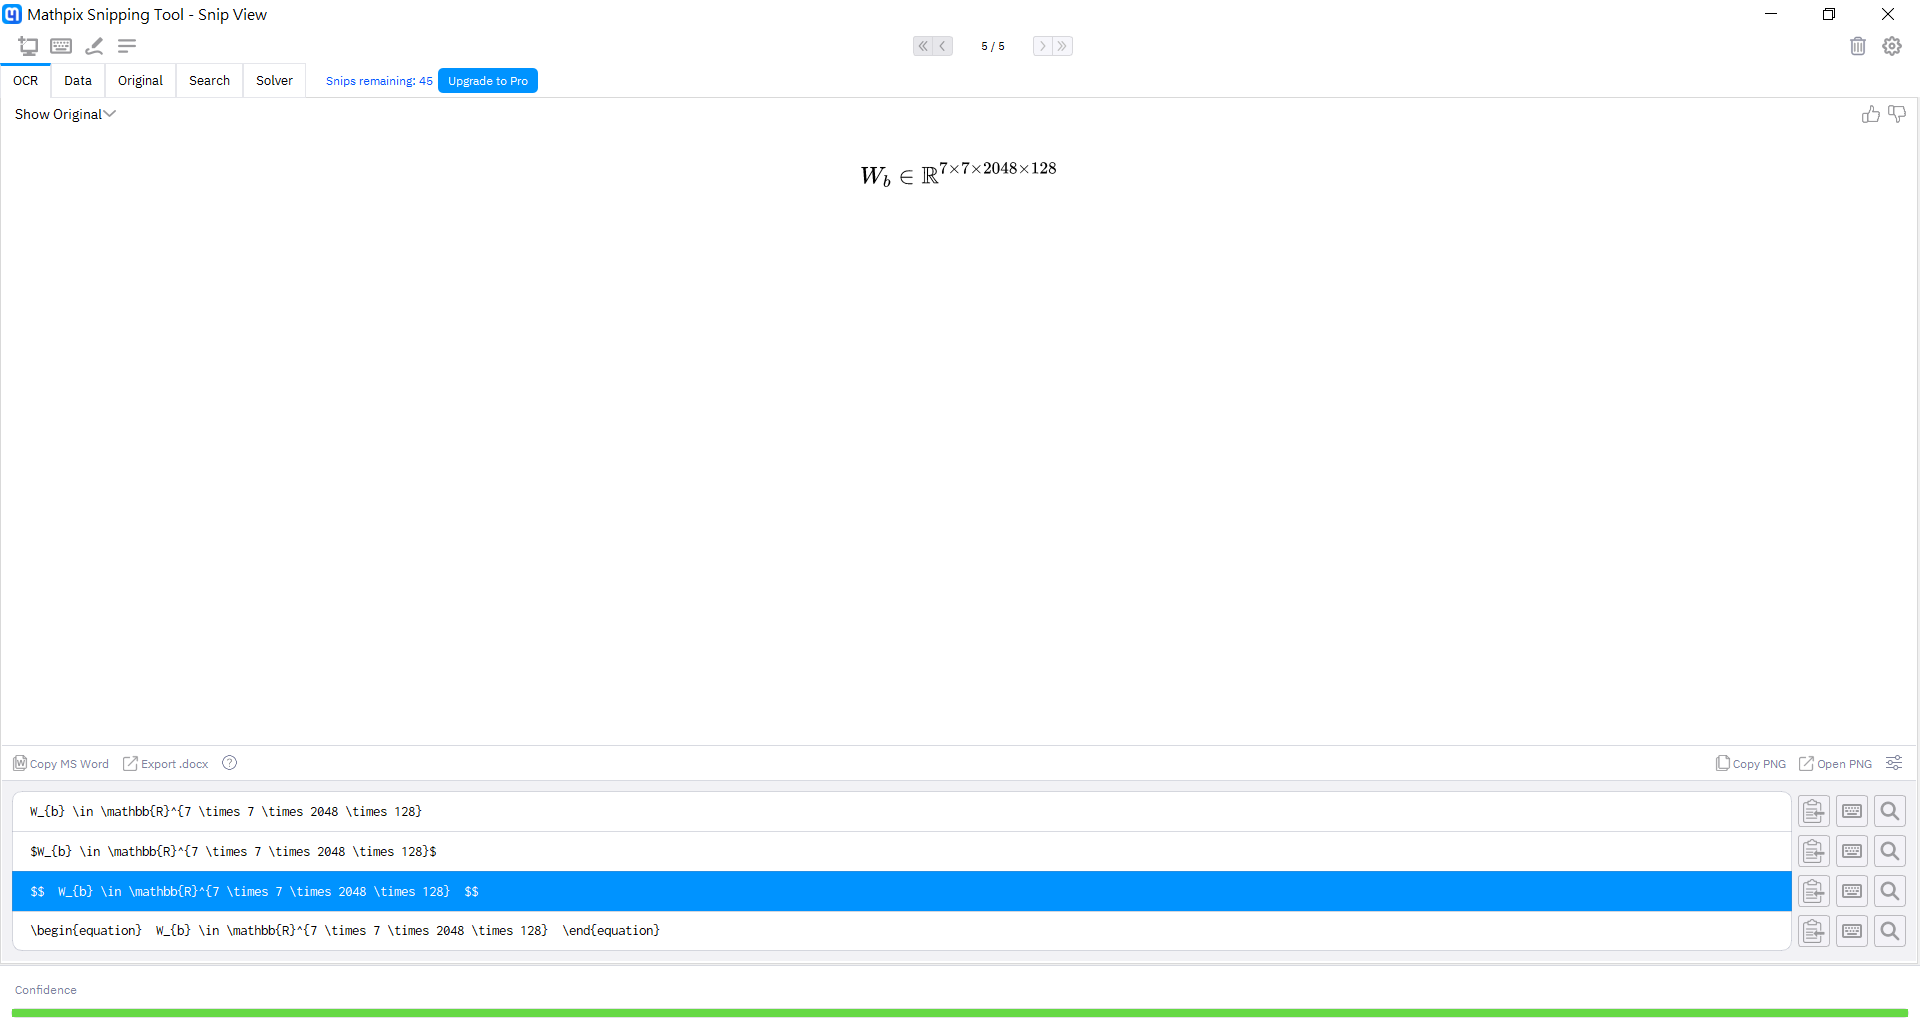
\includegraphics[width=0.90\textwidth]{img/c3m4.png} 
\caption{LaTeX - Mathpix Snip 數學式 OCR 輸出}
\label{Test}
\end{figure}

\subsection{总结}

此作业经过论文精读与全文翻译,同时也研究在 LaTeX 在不同环境下的两种应对方案,前者为 Texmaker 面对本地端稳定的直觉式开发环境,而后者 Overleaf 择重点在快速开发、降低门槛还有多人协作上的优点,并在过程中接触偏大规模的 LaTeX 撰写与研究,并在过程中了解 LaTeX 实际底层的运作跟环境维护,另外也研究了文献管理软体的操作跟时下主要的文献管理软体的优缺点。最后在搜集文献的过程中获得面对研究方向文献收集的经验。
	\chapter{参考文献搜集}

下列为本次作业所搜集而来的文献表,根据本次作业的 7 项来源进行搜集,其包括 IEEE Transaction/Magazine/Journal、IET (IEE) Proceeding/Magazine/Journal、ACM、Springer、Elsevier、Google 学术、Beidu 学术等,最后明确标示使用的平台搜寻引擎跟文献年份。

\begin{center}
\begin{tabular}{cccc}
\hline
研究者 & 平台 & 来源分类 & 备注年份  \\
\hline
Yingkun Xu et al. \cite{yingkunxu2019} & Baidu Scholar & IET (IEE) Proceeding & 2019 \\
Qin Wu et al. \cite{qinwu2020} & Baidu Scholar & IET (IEE) Proceeding & 2020 \\
Abimael Guzmán Pando et al. \cite{abimael2020} & Baidu Scholar & IET (IEE) Proceeding & 2020 \\
Sarah Ahmed et al. \cite{sarahahmed2020} & Baidu Scholar & IET (IEE) Proceeding & 2020 \\
Francisco Luongo et al. \cite{franciscoluongo2020} & Baidu Scholar & IET (IEE) Proceeding & 2020 \\
\hline
\end{tabular}
\end{center}

\begin{center}
\begin{tabular}{cccc}
\hline
研究者 & 平台 & 来源分类 & 备注年份  \\
\hline
Huiyun Gong et al. \cite{huiyungong2021} & Google Scholar & IET (IEE) Proceeding & 2021 \\
Iman Iraei et al. \cite{imaniraei2021} & Google Scholar & IET (IEE) Proceeding & 2021 \\
Yuling Xing et al. \cite{yulingxing2021} & Google Scholar & IET (IEE) Proceeding & 2021 \\
Na Zhu et al. \cite{nazhu2021} & Google Scholar & IET (IEE) Proceeding & 2021 \\
Mohammad Ali Amirabadi et al. \cite{mohammadaliamirabadi2021} & Google Scholar & IET (IEE) Proceeding & 2021 \\
Yanlin Wu et al. \cite{yanlinwu2021} & Google Scholar & IET (IEE) Proceeding & 2021 \\
Jiawei Nian et al. \cite{jiaweinian2021} & Google Scholar & IET (IEE) Proceeding & 2021 \\
Zhao Zhen et al. \cite{zhaozhen2021} & Google Scholar & IET (IEE) Proceeding & 2021 \\
Olarewaju Mubashiru Lawal et al. \cite{olarewaju2021} & Google Scholar & IET (IEE) Proceeding & 2021 \\
Guanwen Zhang et al. \cite{guanwenzhang2021} & Google Scholar & IET (IEE) Proceeding & 2021 \\
Azka Wani et al. \cite{azkawani2021} & Google Scholar & IET (IEE) Proceeding & 2021 \\
Hongxin Ji et al. \cite{hongxinji2021} & Google Scholar & IET (IEE) Proceeding & 2021 \\
Junpeng Wu et al. \cite{junpengwu2021} & Google Scholar & IET (IEE) Proceeding & 2021 \\
Chengxu Ma et al. \cite{chengxuma2021} & Google Scholar & IET (IEE) Proceeding & 2021 \\
Mukesh Kumar Tripathi et al. \cite{mukeshkumar2021} & Google Scholar & IET (IEE) Proceeding & 2021 \\
\hline
\end{tabular}
\end{center}

\begin{center}
\begin{tabular}{cccc}
\hline
研究者 & 平台 & 来源分类 & 备注年份  \\
\hline
Wei Liang et al. \cite{weiliang2021} & ACM & ACM Library & 2021 \\
Wu Q et al. \cite{wuq2021} & ACM & ACM Library & 2021 \\
Chiyuan Zhang et al. \cite{chiyuanzhang2021} & ACM & ACM Library & 2021 \\
Kaixuan Chen et al. \cite{kaixuanchen2021} & ACM & ACM Library & 2021 \\
Shervin Minaee et al. \cite{shervinminaee2021} & ACM & ACM Library & 2021 \\
Guansong Pang et al. \cite{guansongpang2021} & ACM & ACM Library & 2021 \\
Garvit Goel et al. \cite{garvitgoel2021} & ACM & ACM Library & 2021 \\
Tom van der Weide et al. \cite{tomvanderweide2017} & ACM & ACM Library & 2021 \\
Abdul Wasay et al. \cite{abdulwasay2021} & ACM & ACM Library & 2021 \\
Matthew Kusz et al. \cite{matthewkusz2021} & ACM & ACM Library & 2021 \\
\hline
\end{tabular}
\end{center}

\begin{center}
\begin{tabular}{cccc}
\hline
研究者 & 平台 & 来源分类 & 备注年份  \\
\hline
Hironobu Fujiyoshi et al. \cite{fujiyoshi2021} & ScienceDirect & Elsevier & 2021 \\
Geert Litjens PhD et al. \cite{geertlitjens2019} & ScienceDirect & Elsevier & 2019 \\
George Onoufriou et al. \cite{george2019} & ScienceDirect & Elsevier & 2019 \\
A.Inés et al. \cite{aines2019} & ScienceDirect & Elsevier & 2019 \\
Jihoon Oh et al. \cite{jihoonoh2019} & ScienceDirect & Elsevier & 2019 \\
\hline
\end{tabular}
\end{center}

\begin{center}
\begin{tabular}{cccc}
\hline
研究者 & 平台 & 来源分类 & 备注年份  \\
\hline
Carole H. Sudre et al. \cite{carole2017} & Springer & Springer Link & 2017 \\
Mohammad Hesam Hesamian et al. \cite{hesamian2019} & Springer & Springer Link & 2019 \\
Pim Moeskops et al. \cite{pimmoeskops2016} & Springer & Springer Link & 2016 \\
Niall O’Mahony et al. \cite{niall2019} & Springer & Springer Link & 2019 \\
Huazhu Fu et al. \cite{huazhufu2016} & Springer & Springer Link & 2016 \\
\hline
\end{tabular}
\end{center}

\begin{center}
\begin{tabular}{cccc}
\hline
研究者 & 平台 & 来源分类 & 备注年份  \\
\hline
Sarah Adel Bargal et al. \cite{sarahadel2021} & Google Scholar & IEEE Transactions & 2021 \\
Xu Yang et al. \cite{xuyang2021} & Google Scholar & IEEE Transactions & 2021 \\
Mingjie Sun et al. \cite{mingjie2021} & Google Scholar & IEEE Transactions & 2021 \\
Piotr Koniusz et al. \cite{piotr2021} & Google Scholar & IEEE Transactions & 2021 \\
Jianfeng Dong et al. \cite{jianfeng2021} & Google Scholar & IEEE Transactions & 2021 \\
Aysegul Dundar et al. \cite{aysegul2021} & Google Scholar & IEEE Transactions & 2021 \\
Yulin Wang et al. \cite{yulin2021} & Google Scholar & IEEE Transactions & 2021 \\
Lucas Zimmer et al. \cite{lucas2021} & Google Scholar & IEEE Transactions & 2021 \\
Maosen Li et al. \cite{maosen2021} & Google Scholar & IEEE Transactions & 2021 \\
Yang Zhang et al. \cite{yang2021} & Google Scholar & IEEE Transactions & 2021 \\
Kaiyang Zhou et al. \cite{kaiyang2021} & Google Scholar & IEEE Transactions & 2021 \\
Kai Zhao et al. \cite{kaizhao2021} & Google Scholar & IEEE Transactions & 2021 \\
Piotr Koniusz et al. \cite{piotrkoniusz2021} & Google Scholar & IEEE Transactions & 2021 \\
Wenguan Wang et al. \cite{wenguan2021} & Google Scholar & IEEE Transactions & 2021 \\
Xiangbo Shu et al. \cite{xiangbo2021} & Google Scholar & IEEE Transactions & 2021 \\
Wenguan Wang et al. \cite{tianfeizhou2021} & Google Scholar & IEEE Transactions & 2021 \\
Jun Ma et al. \cite{junma2021} & Google Scholar & IEEE Transactions & 2021 \\
Jibin Wu et al. \cite{jibinwu2021} & Google Scholar & IEEE Transactions & 2021 \\
Zhihua Wang et al. \cite{zhihuawang2021} & Google Scholar & IEEE Transactions & 2021 \\
Linjiang Huang et al. \cite{linjiang2021} & Google Scholar & IEEE Transactions & 2021 \\
Nicolas Gillis et al. \cite{nicolasgillis2021} & Google Scholar & IEEE Transactions & 2021 \\
Zhi-Hao Lin et al. \cite{zhihaolin2021} & Google Scholar & IEEE Transactions & 2021 \\
Guohao Li et al. \cite{guohaoli2021} & Google Scholar & IEEE Transactions & 2021 \\
Keren Fu et al. \cite{kerenfu2021} & Google Scholar & IEEE Transactions & 2021 \\
Elvin Isufi et al. \cite{elvinisufi2021} & Google Scholar & IEEE Transactions & 2021 \\
Yawei Luo et al. \cite{yaweiluo2021} & Google Scholar & IEEE Transactions & 2021 \\
Jiangliu Wang et al. \cite{jiangliuwang2021} & Google Scholar & IEEE Transactions & 2021 \\
Mehdi Ali et al. \cite{mehdiali2021} & Google Scholar & IEEE Transactions & 2021 \\
Lin Wang et al. \cite{linwang2021} & Google Scholar & IEEE Transactions & 2021 \\
Xiaosong Zhang et al. \cite{xiaosongzhangfangwan2021} & Google Scholar & IEEE Transactions & 2021 \\
\hline
\end{tabular}
\end{center}


\begin{center}
\begin{tabular}{cccc}
\hline
研究者 & 平台 & 来源分类 & 备注年份  \\
\hline
Filippo Maria Bianchi et al. \cite{filippo2021} & IEEE Xplore & IEEE Transactions & 2021 \\
Xingang Pan et al. \cite{xingang2021} & IEEE Xplore & IEEE Transactions & 2021 \\
Shervin Minaee et al. \cite{shervin2021} & IEEE Xplore & IEEE Transactions & 2021 \\
Xuan Zhang et al. \cite{xuan2021} & IEEE Xplore & IEEE Transactions & 2021 \\
Rui Zhang et al. \cite{rui2021} & IEEE Xplore & IEEE Transactions & 2021 \\
Hongyang Gao et al. \cite{hongyang2021} & IEEE Xplore & IEEE Transactions & 2021 \\
Kai Zhang et al. \cite{kai2021} & IEEE Xplore & IEEE Transactions & 2021 \\
Ke Yu et al. \cite{ke2021} & IEEE Xplore & IEEE Transactions & 2021 \\
Zilong Huang et al. \cite{zilong2021} & IEEE Xplore & IEEE Transactions & 2021 \\
Ming-Kun Xie et al. \cite{mingkun2021} & IEEE Xplore & IEEE Transactions & 2021 \\
Chaoyou Fu et al. \cite{chaoyou2021} & IEEE Xplore & IEEE Transactions & 2021 \\
Mang Ye et al. \cite{mang2021} & IEEE Xplore & IEEE Transactions & 2021 \\
Hongshuang Zhang et al. \cite{hongshuang2021} & IEEE Xplore & IEEE Transactions & 2021 \\
Hanqing Chao et al. \cite{hanqing2021} & IEEE Xplore & IEEE Transactions & 2021 \\
Zerong Zheng et al. \cite{zerong2021} & IEEE Xplore & IEEE Transactions & 2021 \\
Lei Cai et al. \cite{lei2021} & IEEE Xplore & IEEE Transactions & 2021 \\
Xuanyi Dong et al. \cite{xuanyi2021} & IEEE Xplore & IEEE Transactions & 2021 \\
Xinyu Chen et al. \cite{xinyu2021} & IEEE Xplore & IEEE Transactions & 2021 \\
Mathew Monfort et al. \cite{mathew2021} & IEEE Xplore & IEEE Transactions & 2021 \\
Deng-Ping Fan et al. \cite{dengping2021} & IEEE Xplore & IEEE Transactions & 2021 \\
Joey Tianyi Zhou et al. \cite{joeytianyi2021} & IEEE Xplore & IEEE Transactions & 2021 \\
Zhentao Tan et al. \cite{zhentao2021} & IEEE Xplore & IEEE Transactions & 2021 \\
Zhichao Lu et al. \cite{zhichao2021} & IEEE Xplore & IEEE Transactions & 2021 \\
Yi Liu et al. \cite{yi2021} & IEEE Xplore & IEEE Transactions & 2021 \\
Jie Mei et al. \cite{jie2021} & IEEE Xplore & IEEE Transactions & 2021 \\
Adnan Siraj Rakin et al. \cite{adnansiraj2021} & IEEE Xplore & IEEE Transactions & 2021 \\
Jiayuan Li et al. \cite{jiayuan2021} & IEEE Xplore & IEEE Transactions & 2021 \\
Gan Sun et al. \cite{gan2021} & IEEE Xplore & IEEE Transactions & 2021 \\
Jian Liang et al. \cite{jian2021} & IEEE Xplore & IEEE Transactions & 2021 \\
Deng-Bao Wang et al. \cite{dengbao2021} & IEEE Xplore & IEEE Transactions & 2021 \\
\hline
\end{tabular}
\end{center}




    
    \appendix
    \printbibliography[heading = bibintoc]
    
    % 如有需要使用研究生成果页
    \def\cpublication{攻读硕士期间发表的论文及其他成果}

%\renewcommand{\bibname}{\cpublication}
%\begin{thebibliography}{9}{
%\zihao{5}
%\bibitem{publish} 
%\textbf{扎克·施耐德}, XXX XXX, et al. XXXX Title[C/OL]//III H D, SINGH A. Proceedings of Machine Learning Research: Proceedings of the 37th International Conference on Machine Learning: vol. 119. [S.l.]: PMLR, 2020: XXXX-XXXX. http://proceedings.ml r.press/XXXX.html.(一作,CCF-A)
%}\end{thebibliography}
%\addcontentsline{toc}{chapter}{\cpublication}


	\backmatter
	\chapter{致谢}

....
	% 需替换门户原创页pdf/扫描pdf
	%% Copyright (c) 2008-2009 solvethis
% Copyright (c) 2010-2017,2021 Casper Ti. Vector
% Copyright (c) 2021 Kurapica
% Copyright (c) 2021 iofu728
% All rights reserved.
%
% Redistribution and use in source and binary forms, with or without
% modification, are permitted provided that the following conditions are
% met:
%
% * Redistributions of source code must retain the above copyright notice,
%   this list of conditions and the following disclaimer.
% * Redistributions in binary form must reproduce the above copyright
%   notice, this list of conditions and the following disclaimer in the
%   documentation and/or other materials provided with the distribution.
% * Neither the name of Peking University nor the names of its contributors
%   may be used to endorse or promote products derived from this software
%   without specific prior written permission.
%
% THIS SOFTWARE IS PROVIDED BY THE COPYRIGHT HOLDERS AND CONTRIBUTORS "AS
% IS" AND ANY EXPRESS OR IMPLIED WARRANTIES, INCLUDING, BUT NOT LIMITED TO,
% THE IMPLIED WARRANTIES OF MERCHANTABILITY AND FITNESS FOR A PARTICULAR
% PURPOSE ARE DISCLAIMED. IN NO EVENT SHALL THE COPYRIGHT HOLDER OR
% CONTRIBUTORS BE LIABLE FOR ANY DIRECT, INDIRECT, INCIDENTAL, SPECIAL,
% EXEMPLARY, OR CONSEQUENTIAL DAMAGES (INCLUDING, BUT NOT LIMITED TO,
% PROCUREMENT OF SUBSTITUTE GOODS OR SERVICES; LOSS OF USE, DATA, OR
% PROFITS; OR BUSINESS INTERRUPTION) HOWEVER CAUSED AND ON ANY THEORY OF
% LIABILITY, WHETHER IN CONTRACT, STRICT LIABILITY, OR TORT (INCLUDING
% NEGLIGENCE OR OTHERWISE) ARISING IN ANY WAY OUT OF THE USE OF THIS
% SOFTWARE, EVEN IF ADVISED OF THE POSSIBILITY OF SUCH DAMAGE.

{
	\ctexset{section = {
		format+ = {\centering}, beforeskip = {40bp}, afterskip = {15bp}
	}}
	\specialchap{北京大学学位论文原创性声明和使用授权说明}

	% 学校书面要求本页面不要页码,但在给出的 Word 模版中又有页码。
	% 此处以学校书面要求为准。
	\thispagestyle{empty}
	
	% 替换扫描pdf,去除includegraphics前注释
	\begin{textblock}{1}(-0.8,-0.08)
		\colorbox{white}{
			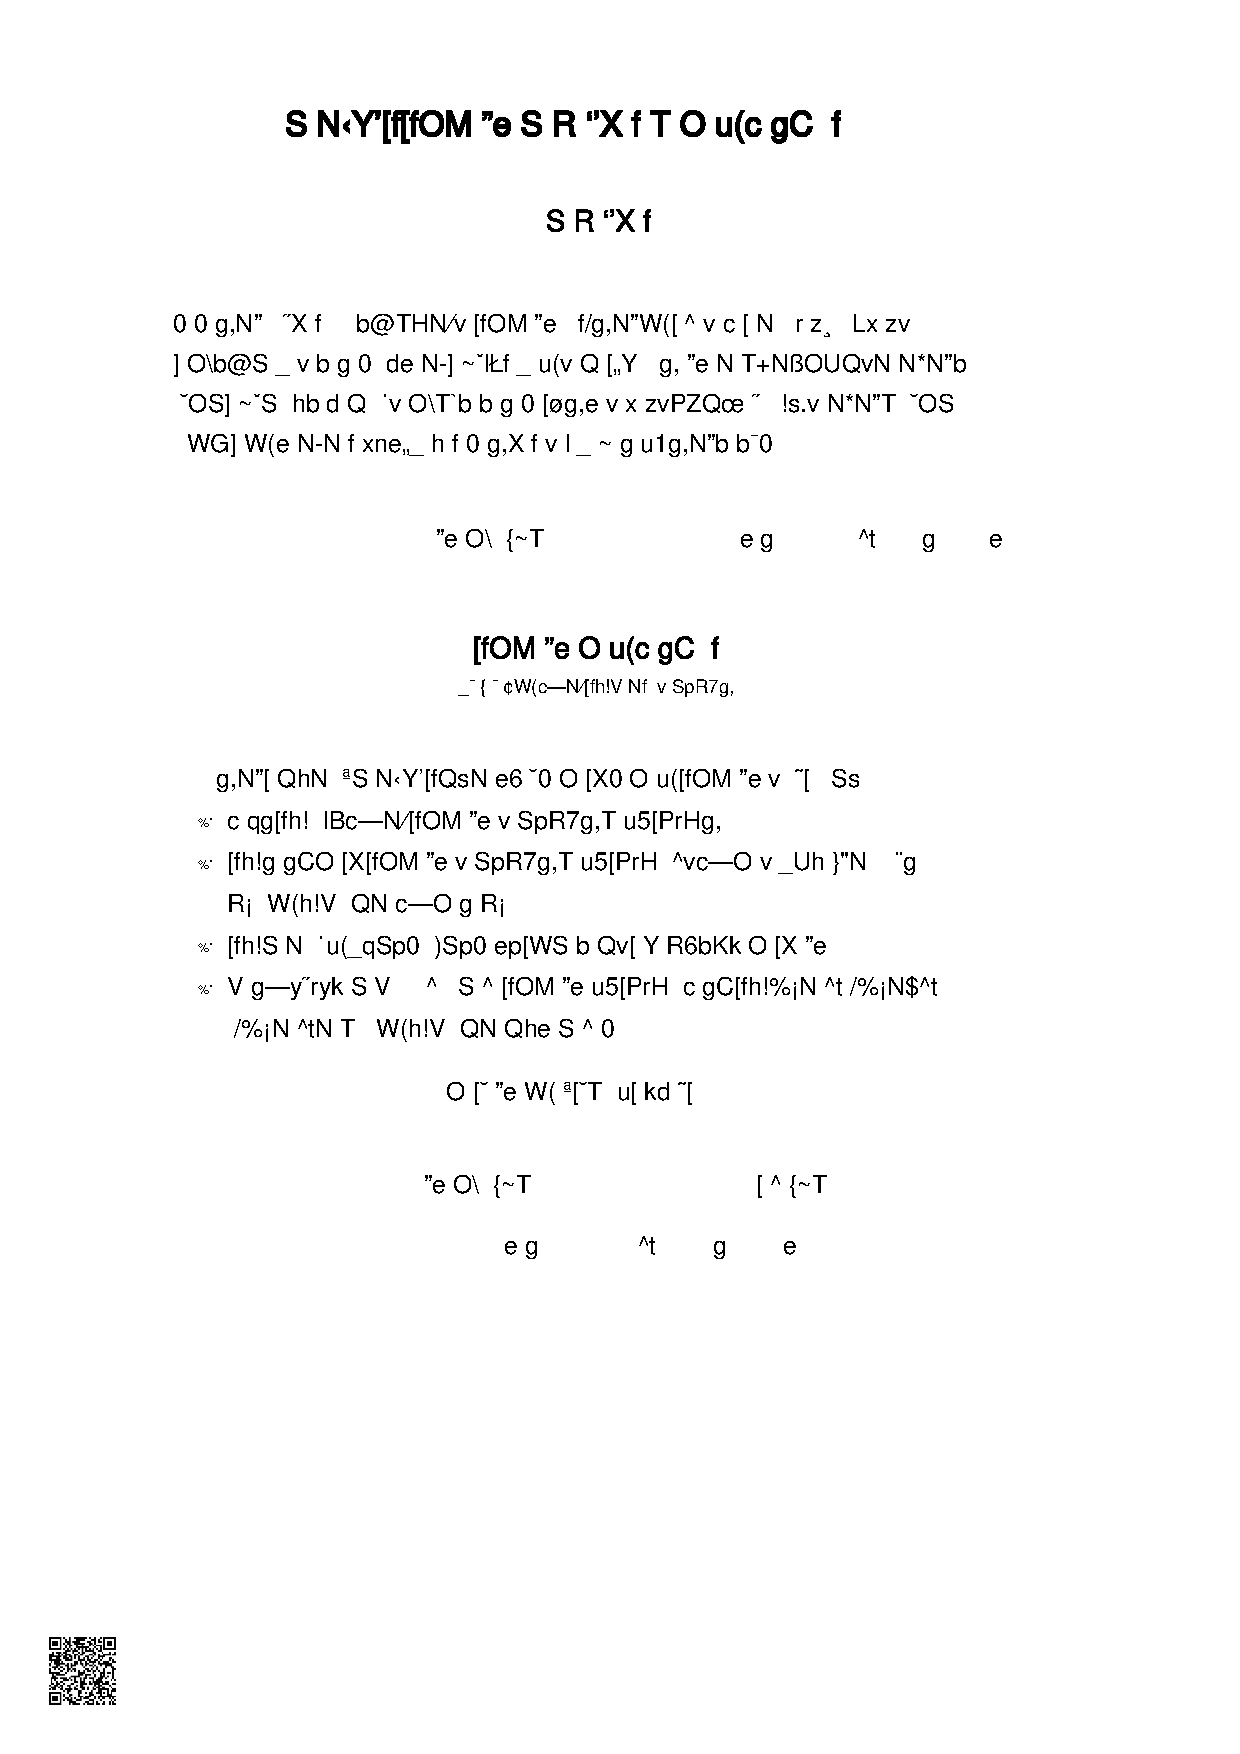
\includegraphics[height = 1.2448\textheight]{img/lwsm_180xxxxxxx.pdf}
		}
	\end{textblock}
}

% vim:ts=4:sw=4

\end{document}

% vim:ts=4:sw=4